\documentclass{mp}
\graphicspath{{03_aksjomatyka/}}
\subtitle{Aksjomatyka rachunku prawdopodobieństwa}
\begin{document}
\frame{\titlepage}
\begin{frame}{Zjawiska losowe i deterministyczne}
\begin{center}
\begin{tikzpicture}[every node/.style={diagram}]
\node (w) {zbiór warunków}
	child { node (det) [below left=of w.center] {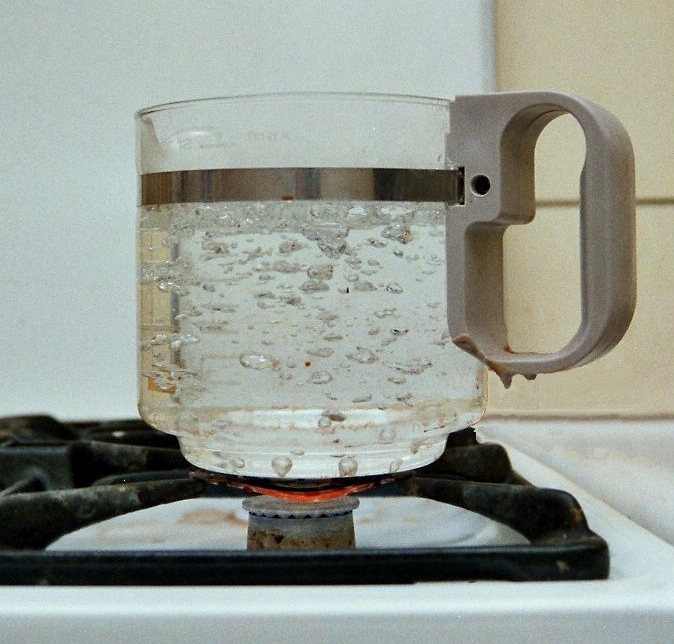
\includegraphics[width=.3\textwidth] {Kochendes_wasser02.jpg}}}
	child { node (los) [below right=of w.center] {\includegraphics[width=.3\textwidth] {head.jpg}}};
\end{tikzpicture}
\end{center}
\vfill
{\tiny Zdjęcie wody z \url{http://commons.wikimedia.org/wiki/File:Kochendes_wasser02.jpg} by \emph{Markus Schweiss} CC-BY-SA-3.0\\
Zdjecie monety z \url{http://commons.wikimedia.org/wiki/File:Powstanie_listopadowe_5_z\%C5\%82otych_1831.JPG} by \emph{Niki K} CC BY-SA 3.0}
\end{frame}
\begin{frame}{Zdarzenia}

\[\only<3>{\Omega=\{\omega_1, \omega_2, \omega_3, \omega_4, \omega_5, \omega_6\}}\] \[\only<4>{A=\{\omega_1, \omega_4, \omega_5\} \qquad B=\{\omega_2, \omega_5\}}\]
\begin{center}
\begin{tikzpicture}[dice/.style={draw=black,thick,rectangle,minimum size=10mm,diagram},
every token/.style={top color=black, bottom color=black, semitransparent}]
\node (d1) [dice,tokens=1] 		{} node[visible on=<2->] (d1label) at ($(d1.south)-(0,.15)$) {$\omega_1$};
\node (d2) [dice,tokens=2,right=of d1]  {} node[visible on=<2->] (d2label) at ($(d2.south)-(0,.15)$) {$\omega_2$};
\node (d3) [dice,tokens=3,right=of d2]  {} node[visible on=<2->] (d3label) at ($(d3.south)-(0,.15)$) {$\omega_3$};
\node (d4) [dice,tokens=4,below=of d1]  {} node[visible on=<2->] (d4label) at ($(d4.north)+(0,.15)$) {$\omega_4$};
\node (d5) [dice,tokens=5,right=of d4]  {} node[visible on=<2->] (d5label) at ($(d5.north)+(0,.15)$) {$\omega_5$};
\node (d6) [dice,tokens=6,right=of d5]  {} node[visible on=<2->] (d6label) at ($(d6.north)+(0,.15)$) {$\omega_6$};
\coordinate (center) at ($.5*(d2.south)+.5*(d5.north)$);
%\begin{scope}[visible on=<2>]
%\path ($(center)-(6cm,0)$) node[align=center] (elementarne) {zdarzenia\\elementarne};
%\foreach \label in {d1label, d2label, d3label, d4label, d5label, d6label}
%	\draw[->,set,draw=black] (elementarne.east) -- (\label);
%\end{scope}
\draw [set,color1,visible on=<3->] (center)  circle [x radius=40mm, y radius=31mm] node (omegalabel) at ($(center)-(43mm,0)$) {$\Omega$};
%\path [visible on=<3>,->,set,draw=black] ($(omegalabel)-(3cm,1cm)$) node[align=center] (pze) {przestrzeń\\zdarzeń\\elementarnych} (pze) -- (omegalabel);
\draw [set,color2,visible on=<4>] ($(d1.west)-(2mm,0)$) |- ($(d1.east)+(2mm,7mm)$) |- ($(d5.east)+(2mm,7mm)$) |- ($(d4.west)-(2mm,7mm)$) -- cycle node (A) at ($.5*(d1.south)+.5*(d4.north)$) {$A$};
\draw [set,color3,visible on=<4>] ($(d2.west)-(2mm,0)$) |- ($(d2.east)+(3mm,7mm)$) |- ($(d5.west)-(2mm,8mm)$)  -- cycle node (B) at (center) {$B$};
%\begin{scope}[visible on=<4>]
%\path ($(A)-(5cm,-1cm)$) node[align=center] (zdarzenia) {zdarzenia};
%\draw[->,set,draw=black] (zdarzenia) -- (A);
%\draw[->,set,draw=black] (zdarzenia) -- (B);
%\end{scope}
\end{tikzpicture}
\end{center}
\end{frame}

\begin{frame}{Działania na zdarzeniach}
\begin{center}
\begin{tikzpicture}
\draw [name path=O,set,color1] (0,0)  circle (35mm);
\begin{scope}[visible on=<2-6>]
\draw [name path=A,set,color2] (-2cm,-1cm) rectangle (1cm,1cm) node at (-1.5cm,0) {$A$};
\draw [name path=B,set,color3,visible on=<2>] (-.75cm,-.75cm) rectangle (.75cm,.75cm) node at (0,0) {$B$};
\begin{scope}[visible on=<3-4>]
\draw [name path=B,set,color3] (-.75cm,-.75cm) rectangle (1.25cm,2cm) node at (0,1.5cm) {$B$};
\fill [pattern=crosshatch,pattern color=color4,visible on=<3>,name intersections={of=A and B}] (intersection-1) rectangle (intersection-2);
\fill [pattern=crosshatch,pattern color=color4,visible on=<4>,name intersections={of=A and B,sort by=A}] (-2cm,-1cm) |- (intersection-1) |- (1.25cm,2cm) |- (intersection-2) |- (-2cm,-1cm) -- cycle;
\end{scope}
\draw [name path=B,set,color3,visible on=<5>] (-.5cm,1.25cm) rectangle ++(2cm,1.75cm) node at (0.75cm,2.3cm) {$B$};
\node [color3,visible on=<6>] at (0,2.5cm) {$A'$};
\end{scope}
\begin{scope}[visible on=<7>]
\draw [name path=A,set,color2] (0,0) -- (30:35mm);
\draw [name path=B,set,color3] (0,0) -- (135:35mm);
\draw [name path=C,set,color4] (0,0) -- (290:35mm);
\node [color2] at (0,2cm) {$A$};
\node [color3] at (-2cm,0) {$B$};
\node [color4] at (2cm,0) {$C$};
\end{scope}
\end{tikzpicture}
\end{center}
\end{frame}

\begin{frame}{Przestrzeń probabilistyczna}
\[(\Omega,\mathcal{A},P)\]

\begin{center}
\begin{tikzpicture}
\node[diagram] (root) {$\left|\Omega\right|$}
	child { node [diagram,below left=of root.center] {$\mathcal{A}=2^\Omega$} edge from parent node[left] {$\leq\left|\mathbb{N}\right|$}}
	child { node [diagram,below right=of root.center] {$\mathcal{A}\subset 2^\Omega$} edge from parent node[right] {$=\left|\mathbb{R}\right|$}};
\end{tikzpicture}
\end{center}
\end{frame}

\begin{frame}{Aksjomaty Kołmogorowa}
\begin{minipage}{.6\textwidth}
\begin{enumerate}
\item \[P\colon \mathcal{A} \to \left[0;1\right]\]
\item \[P(\Omega)=1\]
\item dla dowolnego, najwyżej przeliczalnego ciągu rozłącznych zdarzeń $A_1, A_2, \ldots \in \mathcal{A}$: \[ P(A_1\cup A_2\cup \ldots)=P(A_1)+P(A_2)+\ldots\]
\end{enumerate}
\end{minipage}
\begin{minipage}{.39\textwidth}
\centering 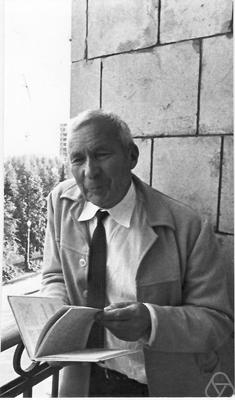
\includegraphics[width=\textwidth,clip,viewport=0 0 10cm 11cm]{kolmogorov.jpg} \\
Andriej Kołmogorow (1903--1987) \\
{\tiny \url{http://owpdb.mfo.de/detail?photo_id=7493} CC BY-SA 2.0 DE}
\end{minipage}
\end{frame}

\begin{frame}{Różne podejścia do $P$}
\begin{center}
\only<1>
{
	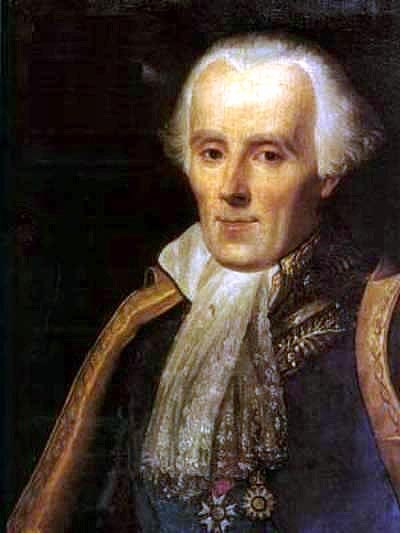
\includegraphics[height=.7\textheight]{Pierre-Simon_Laplace.jpg} \\
	Pierre Simon de Laplace (1749--1827)\\
	{\tiny \url{http://commons.wikimedia.org/wiki/File:Pierre-Simon_Laplace.jpg}, domena publiczna}
}
\only<2>
{
	\begin{tikzpicture}[dice/.style={draw=black,thick,rectangle,minimum size=10mm,diagram,node distance=2mm},
		every token/.style={top color=black, bottom color=black, semitransparent}]
		\node (d1) [dice,tokens=1] 		{};
		\node (d2) [dice,tokens=2,right=of d1]  {};
		\node (d3) [dice,tokens=3,right=of d2]  {};
		\node (d4) [dice,tokens=4,right=of d3]  {};
		\node (d5) [dice,tokens=5,right=of d4]  {};
		\node (d6) [dice,tokens=6,right=of d5]  {};
		\node (x2) [dice,tokens=2,above=5mm of d2]  {};
		\node (x4) [dice,tokens=4,above=5mm of d4]  {};
		\draw [very thick] ($(d1.west)+(-3mm,7.5mm)$) -- ($(d6.east)+(3mm,7.5mm)$);
%		\foreach \x in {d1,x2}
%			\draw [very thick] ($(\x.west)+(-1.5mm,6mm)$) -- ++(0,-12mm);
%		\foreach \x in {d6,x4}
%			\draw [very thick] ($(\x.east)+(1.5mm,6mm)$) -- ++(0,-12mm);
	\end{tikzpicture}
}
\only<3>
{
	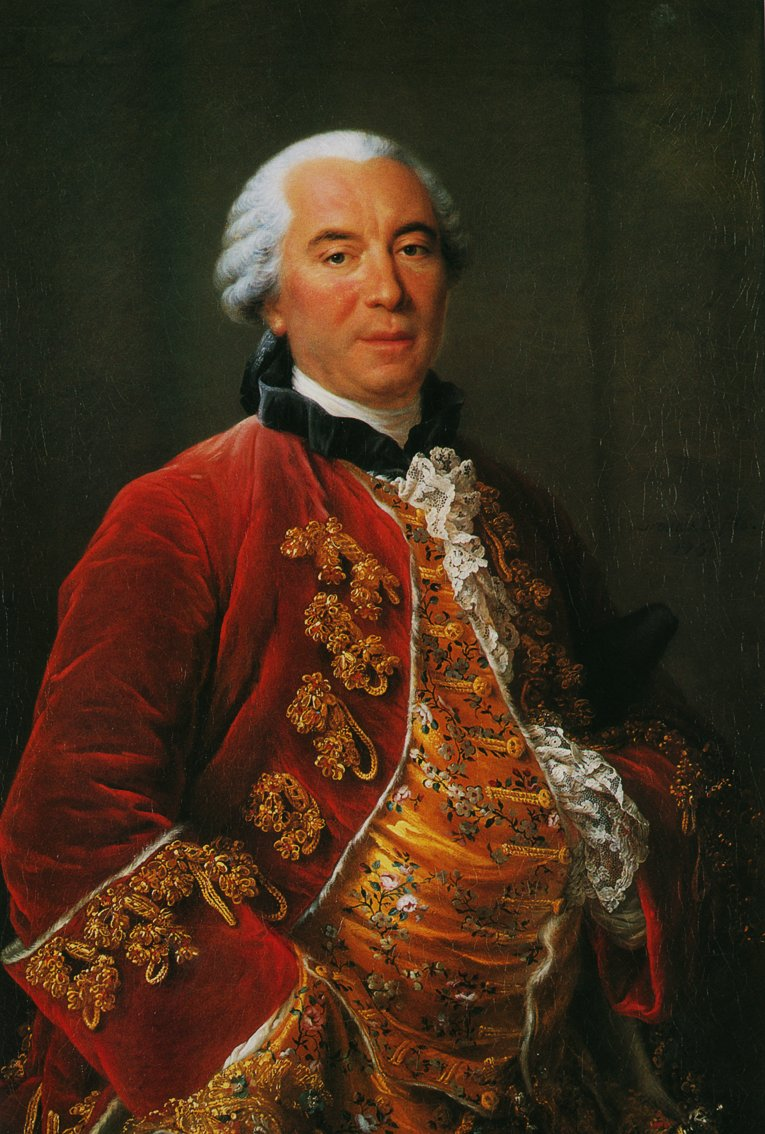
\includegraphics[height=.7\textheight]{Buffon_1707-1788.jpg}\\
	Georges-Louis Leclerc, Comte de Buffon (1707--1788)\\
	{\tiny \url{http://commons.wikimedia.org/wiki/File:Buffon_1707-1788.jpg}, domena publiczna}
}
\only<4>
{
	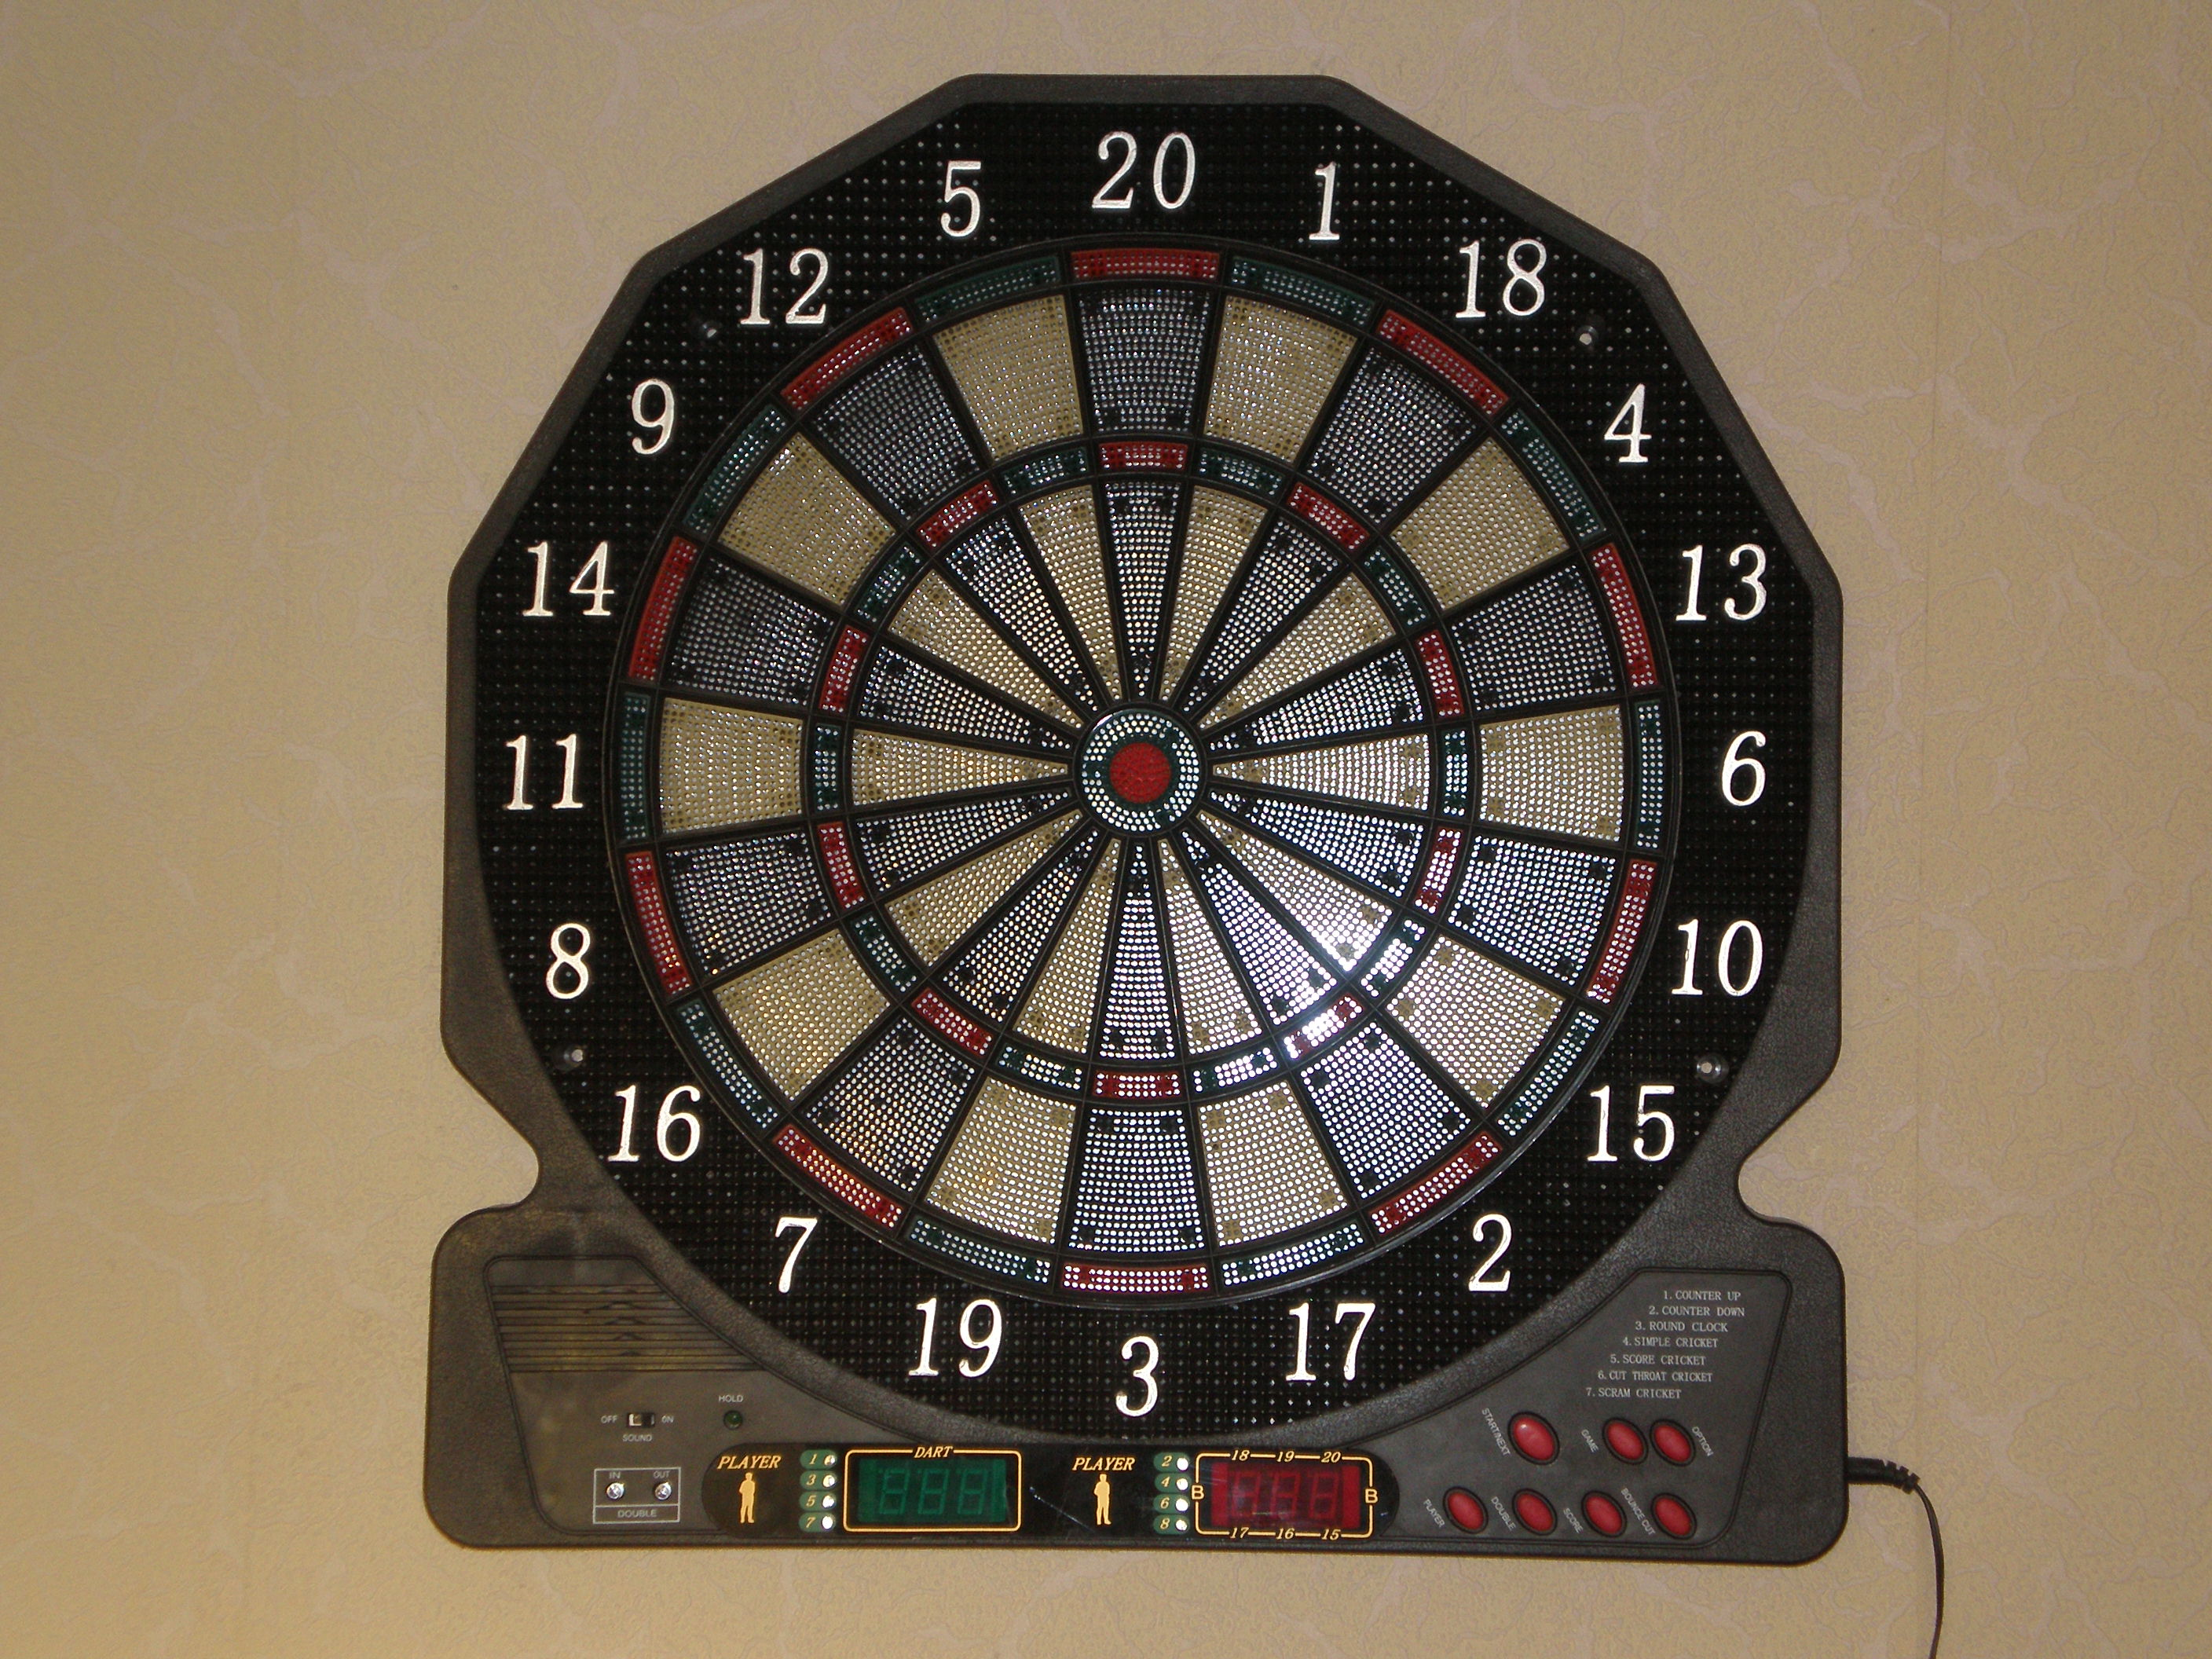
\includegraphics[height=.7\textheight]{Electronic_dart_board.jpg}\\
	{\tiny \url{http://commons.wikimedia.org/wiki/File:Electronic_dart_board.jpg} by Krzysztof Szymański CC BY 2.5}
}
\end{center}
\end{frame}

\begin{frame}{Przykład prawdopodobieństwa geometrycznego}
\centering
\begin{tikzpicture}
\draw (0,0) circle [radius=3cm];
\draw (0,0) -- (-3,0) node[near end,above] {3cm};
\draw[color=cegla] (0,0) circle [radius=1.5cm];
\draw (0,0) -- (0,1.5) node[midway,above] {$1{,}5$ cm};
\node[color=cegla] at (-1.3,1.3) {A};
\node at (-2.3,2.3) {$\Omega$};
\end{tikzpicture}
\[P(\textcolor{cegla}{A})=\alert{?}\]
\end{frame}

\begin{frame}{Przydatne twierdzenie}
	\begin{block}{Twierdzenie}
		Dla dowolnych zdarzeń $A, B$ zachodzi
		\[ P(A\cup B)=P(A)+P(B) - P(A\cap B) \]
	\end{block}
\end{frame}

\begin{frame}{Porównywanie wielomianów}
\only<4>{Ile najwyżej pierwiastków rzeczywistych mają poniższe wielomiany?}
\only<1,2,4,6-8>{
\begin{align*}
% maxima: A(x):=(x-2)^2*(x-4)^2*(x-6)^2*(x-8)^2;
A(x)= & \left(x-8\right)^2\,\left(x-6\right)^2\,\left(x-4\right)^2\,\left(x-2\right)^2 \\
% maxima: B(x):=A(x)-(x-1)*(x-2)*(x-4)*(x-6)*(x-8);
B(x)= & x^8-40\,x^7+680\,x^6-6401\,x^5+36389\,x^4-\\& 127520\,x^3+268060\,x^2-307984\,x+147840\\
% maxima: tex(expand(A(x)));
C(x)= & x^8-40\,x^7+680\,x^6-6400\,x^5+36368\,x^4- \\& 127360\,x^3+267520\,x^2-307200\,x+147456\\
% %maxima: A(x):=(x-1)*(x-2)*(x-3)*(x-4)*(x-5)*(x-6)*(x-7)*(x-8)*(x-9)*(x-10);
% A(x) = &\left(x-10\right)\,\left(x-9\right)\,\left(x-8\right)\,\left(x-7\right)\,\left(x-6\right)\,\left(x-5\right)\,\\
%  & \left(x-4\right)\,\left(x-3\right)\,\left(x-2\right)\,\left(x-1\right) \\
% %maxima: tex(expand(A(x)));
% B(x) = & x^{10}-55\,x^9+1320\,x^8-18150\,x^7+157773\,x^6-902055\,x^5+\\
%  & 3416930\,x^4-8409500\,x^3+12753576\,x^2-10628640\,x+3628800 \\
% %maxima: C(x):=(x-2)*(x-2)*(x-4)*(x-4)*(x-6)*(x-6)*(x-7)*(x-8)*(x-9)*(x-10);
% C(x) = & x^{10}-58\,x^9+1479\,x^8-21798\,x^7+205224\,x^6-1286736\,x^5+\\
%  & 5427056\,x^4-15159392\,x^3+26753280\,x^2-26850816\,x+11612160
\only<4>{A(x)-B(x) = & \ldots \\ A(x)-C(x) = & \ldots}
\end{align*}
\only<2>{
	Jaki jest koszt deterministycznego sprawdzenia czy $A(x)\equiv B(x)$ (w~ogólności oba wielomiany stopnia $n$)?
	%żeby rozwinąć A(x) potrzeba O(n^2) mnożeń
}
\only<6-8>
{
	\begin{align*}
		\only<6->{A(2) &=0 	& B(2) &=0 		& C(2) &=0}\\
		\only<7->{A(1) &=11025 	& B(1) &=11025 		& C(1) &=11025}\\
		\only<8->{A(3) &=225 	& B(3) &=\alert{255} 	& C(3) &=225}\\
	\end{align*}
}
}
\only<3>{
	\begin{block}{Zasadnicze twierdzenie algebry}
		Każdy wielomian stopnia $n>0$ można przedstawić jako iloczyn \[a(x-x_1)(x-x_2)\ldots(x-x_n)\] dla pewnych $a,x_1,\ldots,x_n\in\mathbb{C}$
	\end{block}
}
\only<5>{

	\begin{center}
	\begin{tikzpicture}
	\node[diagram] (root) {$A(x)\equiv B(x)$}
		child { node [diagram,below left=of root.center,align=left] {$A(x)-B(x)\equiv 0$\\$\forall x\in\R\colon A(x)-B(x)=0$} edge from parent node[left] {\cmark}}
		child { node [diagram,below right=of root.center,align=left] {$A(x)-B(x)\not\equiv 0$\\$\exists x\in\R\colon A(x)-B(x)\neq 0$} edge from parent node[right] {\xmark}};
	\end{tikzpicture}
	\end{center}
}
\only<9-11>{
	\[ \Omega = \{ \omega_1, \omega_2, \ldots, \omega_{799}, \omega_{800} \} \]
	\only<10->{\[X = \{\omega_{x_1}, \omega_{x_2}, \ldots, \omega_{x_k} \} \qquad A(x_i)-B(x_i)=0 \qquad k\leq 8 \] \\}
	\only<11->{\[P(X)=\frac{\left|X\right|}{\left|\Omega\right|}\leq\frac{1}{100}\]}
}
\only<12>{
	Koszt obliczeniowy dla wielomianu \ldots
	\begin{itemize}
		\item \ldots w postaci iloczynu, np. $(x-1)(x-2)$? %mnożenie O(1) czyli O(k)
		\item \ldots w postaci kanonicznej, np. $x^2-3x+2$? %szybkie potęgowanie O(log(k)), czyli O(klog(k))
		%ostatecznie O(klog k)<O(k^2)
	\end{itemize}
}
\end{frame}
\end{document}
